%% Documentclass:
\documentclass[OpenMind]{stjour}

%\usepackage{subcaption}
\usepackage{gb4e}

%% Or,

%% Manuscript, for double spaced, larger fonts
% \documentclass[manuscript]{stjour}
%% Only needed if you use `manuscript' option
% \journalname{Open Mind}

%%%%%%%%%%%%%%%%%%%%%%%%%%%%%%%%%%%%%%%%%%%%%%%%%%
%% For production only, not authors:
%%\documentclass[OpenMind,finalfonts]{stjour}

%%%%%%%%%%% Please supply information %%%%%%%%%%%%%%%%%%%%%%%%%

%% For Open Mind:
%% Supplementary Materials:
\supplementslinks{dx.doi.org/10.1098/rsif.2013.0969}

%% If no conflicts, this command doesn't need to be used
%% \conflictsofinterest{}

%%%%%%%%%%% to be supplied by MIT Press, only %%%%%%%%%%%%%%%%%

\citation{XXX}

\received{XXX}
\accepted{XXX}
\published{XXX}

%% DOI address:
\setdoi{XXX}

%%%%%%%% End MIT Press commands %%%%%%%%%%

%%%%%%%%%%%%%%%%%%%%%%%%%%%%%%%%%%%%%%%%%%%%%%%%%%%%%%%%%%%%%%%
%% author definitions should be placed here:


\definecolor{Pink}{RGB}{255,50,170}
\newcommand{\jd}[1]{\textcolor{Pink}{[jd: #1]}}  

\newcommand{\jt}[1]{\textbf{\color{blue}JT: #1}}


\begin{document}

\title{Prior beliefs modulate projection}
%\subtitle{<Subtitle Here>} %% Optional subtitle

%% If shortened title for running head is needed so that the article title can fit
%%   in the running head, use [] argument, ie,
%%
%%   \title[Shortened Title for Running Head]{Title of Article}
%%   \subtitle{Subtitle Here}

%%% Author/Affil
%% Since we use \affil{} in the argument of the \author command, we
%% need to supply another version of the author names, without \affil{}
%% to be used for running heads:

\author[Judith Degen, Judith Tonhauser]
{Judith Degen\affil{1} 
\and Judith Tonhauser\affil{2}}

\affiliation{1}{Department of Linguistics, Stanford University, Stanford, USA}

%ie.
%\affiliation{1}{Gatsby Computational Neuroscience Unit, University
%College London, London, United Kingdom} 

\affiliation{2}{Department of English Linguistics, University of Stuttgart, Stuttgart, Germany}

%ie
%\affiliation{2}{Center for Studies in
%Behavioral Neurobiology, Concordia University, Montreal, Quebec,
%Canada}

\correspondingauthor{Judith Degen}{jdegen@stanford.edu}

% ie,
%\correspondingauthor{Ritwik K. Niyogi}{ritwik.niyogi@gatsby.ucl.ac.uk}

\keywords{experimental semantics, experimental pragmatics, projection}

%ie
%\keywords{work, leisure, normative, microscopic,  reinforcement learning, economics}

\begin{abstract}
Beliefs about the world affect language processing and interpretation in several empirical domains. In two experiments, we tested whether subjective prior beliefs about the probability of utterance content modulate \emph{projection}, that is, listeners' inferences about speaker commitment to that content. We find that prior beliefs predict projection at both the group and the by-participant level: the higher the prior belief in a content, the more speakers are taken to be committed to it. This result motivates the integration of formal analyses of projection with cognitive theories of language understanding.  
\end{abstract}

\section{Introduction}

Psycholinguistic work has documented several ways in which probabilistic beliefs about the world, often termed {\em world knowledge}, affect  language processing  \citep[e.g.,][]{chambers-etal02,hagoort-etal2004,hald-etal2007,warren2007}, including syntactic ambiguity resolution \citep[e.g.,][]{chambers-etal04,bicknell-rohde2009}, reference resolution \citep[e.g.,][]{winograd1972, hanna-tanenhaus04}, genericity \citep[e.g.,][]{tessler-goodman2019},  scalar implicature \citep[e.g.,][]{degen-etal2015}, underinformativity implicatures \citep{kravtchenko2015}, and the production of redundant referring expressions \citep{mitchell2013, westerbeek2015, Rubio2016, DegenEtAl2020, sedivy2003}. In contrast, formal linguistic research on meaning in the tradition of \citet{montague73}, which is devoted to specifying how meanings of expressions are computed from the meanings of the parts of the expressions, the way the parts are combined, and the contexts in which the expressions are used, has often sidelined world knowledge, as non-linguistic, encyclopedic knowledge that must enter into the meaning computation, but whose effect has eluded systematic investigation and  formalization \citep[for relevant discussion see, e.g.][] {dowty86,peeters2000,beaver01,hobbs2019}.\footnote{Because {\em knowledge} implies justified true belief but subjective beliefs need not be accurate to affect language processing in systematic ways, we henceforth avoid the term {\em world knowledge} and instead refer to {\em (subjective prior) beliefs about the world}.}   In this paper, we provide empirical evidence from English that \emph{projection}, a key topic in linguistic research on meaning, is systematically modulated by listeners'\footnote{We include readers, writers, and signers in the terms {\em listener} and {\em speaker}.} subjective beliefs about the world. This provides further impetus for accounts of meaning computation to include a mechanism for integrating subjective prior beliefs. We provide a sketch of such an account at the end of this paper.

To introduce projection, consider first that speakers can present themselves, through their utterances, as believing that particular content is true, that is, as committed to that content. Listeners, in turn, regularly draw inferences about which content speakers present themselves as committed to.  For instance, if a speaker utters \emph{Sam knows that it's raining}, listeners typically infer that the speaker is committed to the following two contents: (i) the content of the complement (CC) of {\em know},  that it's raining; and (ii) the content of the matrix clause, that Sam knows (i). In formal research on meaning, the inference to (i) is attributed to the speaker having uttered the sentence, and the inference to (ii) is attributed to the lexical meaning of {\em know}, specifically, that only true content can be known \citep[e.g.,][]{ccmg90}. The puzzle is that the inference to (i) may persist even when the speaker inquires about what Sam knows, as in {\em Does Sam know that it's raining?}, or when the speaker denies Sam's knowledge, as in {\em Sam doesn't know that it's raining}. Because Sam's knowledge is questioned or even denied in these variants, that is, the inference to (ii) does not persist, these inferences to (i) cannot be attributed to the aforementioned lexical meaning of {\em know}. This phenomenon of speaker commitment to utterance content that occurs in negated sentences or questions is termed \emph{projection}. Decades of research in formal semantics have aimed to explain why content projects \citep[e.g.,][]{langendoen-savin71,beaver-geurts-sep}.

%\jd{JD, update this to be more readable}To introduce projection, consider first that listeners regularly draw inferences about utterance content that speakers are committed to. A speaker is taken to be committed to a content if they publicly behave as though they believe or are certain of that content. For instance, if a speaker utters \emph{Sam knows that it's raining}, listeners typically infer that the speaker is committed to the following two contents: (i) the content of the complement (CC) of {\em know}, i.e.,  that it's raining; and (ii) the content of the matrix clause, i.e., that Sam knows (i). In formal research on meaning, the inference to (i) is attributed to the speaker having asserted the sentence, and the inference to (ii) is attributed to the lexical meaning of {\em know}, specifically, that only true content can be known \citep[e.g.,][]{ccmg90}. The puzzle is that the inference to (ii) persists even when the speaker inquires about what Sam knows, as in {\em Does Sam know that it's raining?}, or when the speaker denies Sam's knowledge, as in {\em Sam doesn't know that it's raining}. Because Sam's knowledge is questioned or even denied in these variants, that is, the inference to (i) does not persist, these inferences to (ii) cannot be attributed to the aforementioned lexical meaning of {\em know}. \jd{upon re-reading, i'm convinced once again that (i) and (ii) must be reversed for this to make sense. let's walk through it tomorrow so you can correct me again. my understanding is that the puzzle is that the inference to (i) persists despite the inference to (ii) not persisting, not the other way around (as it is currently formulated)} This phenomenon of speaker commitment to utterance content that occurs in a negated sentence or a question is termed \emph{projection}. Decades of research in formal semantics have aimed to explain why content projects \citep[e.g.,][]{langendoen-savin71,beaver-geurts-sep}.




While content is standardly taken to either project or not \citep{beaver-geurts-sep}, recent experimental work suggests that projection is gradient: listeners' inferences about speaker commitment to utterance content vary in strength and are modulated by the expression (e.g., {\em know} vs.\ {\em discover} vs.\ {\em announce}) and by contextual factors including the discourse status of the content and the prosody of the utterance \citep[for an overview see][]{tbd-variability}. The hypothesis that listeners' prior beliefs modulate projection was initially put forth by \citet{stevens-etal2017} and \citet{tbd-variability}, who observed by-item projection variability for different CCs of clause-embedding predicates like \emph{know} and \emph{discover}. They argued that one source of the observed variability may be that more a priori likely content ({\em Kim flew to New York}) projects more strongly than less a priori likely content  ({\em Kim flew to the moon}) when realized as the CC of a clause-embedding predicate (as in \emph{Did John discover that Kim flew to New York/the moon?}). This idea can straightforwardly be made sense of under recent Bayesian accounts that treat pragmatic utterance interpretation as a matter of combining uncertain prior beliefs about the world with uncertain beliefs about likely speaker production choices via Bayes' rule \citep{GoodmanFrank2016, degen-etal2015}: a CC that is more likely a priori (\emph{before} observing an utterance) is also more likely a posteriori (\emph{after} observing an utterance).

%\citeNP{stevens-etal2017} investigated the projection of the prejacent of manner adverb sentences; for instance, the content that Masha ran of the negated sentence {\em Masha didn't run quickly}. They hypothesized that the observed by-item variability might be due to prejacents differing in their prior probability and higher prior probability contents being more projective. \citeNP{tbd-variability} investigated the projection of content associated with 19 American English expressions, including the content of the complement of clause-embedding predicates like {\em know}, illustrated in (\ref{know}), and the prejacent of {\em stop}; for instance, the content that Mary's daughter has been biting her nails of the polar question {\em Has Mary's daughter stopped biting her nails?}. These authors, too, hypothesized that prior probability influences projection (p.500), as formulated in the hypothesis in (\ref{hyp}):

%Like \citeNP{stevens-etal2017}, \citealt[500]{tbd-variability} hypothesized that ``the projectivity of content may depend on the prior probability of the event described by the expression that conveys the content, such that content conveyed by expressions that describe more a priori likely events may be more likely to project''.

%\begin{exe}
%\ex\label{stop} Has Mary's daughter stopped biting her nails?
%\begin{xlist}
%\ex Mary's daughter stopped biting her nails.
%\ex Has Mary's daughter stopped biting her nails?
%\end{xlist}
%\end{exe}

%stop nails 0.79
%Has Mary?s daughter stopped biting her nails?
%Mary's daughter has been biting her nails
%stop play 0.89
%Did Jack stop playing outside with the kids?
%Jack was playing outside with the kids


%investigated the projection of the prejacent of utterances of manner adverb sentences, illustrated in (\ref{manner}). An utterance of (\ref{manner}a) implies both the prejacent, that Masha ran, and that her running was done in a quick manner. The prejacent is projective because it may also be implied by an utterance of the negated variant of (\ref{manner}a) given in (\ref{manner}b), especially when the adverb is produced with prosodic emphasis. 
%
%\begin{exe}
%\ex\label{manner} \citealt[1144]{stevens-etal2017}
%\begin{xlist}
%\ex Masha ran quickly.
%\ex Masha didn't run QUICKLY.
%\end{xlist}
%\end{exe}
%\citeNP{stevens-etal2017} observed by-item variability in the projection of the prejacent and suggested that this variability may be due to listeners having different prior probabilities about the prejacent.

% jd commented out:
%\begin{exe}
%\ex\label{hyp} {\bf Hypothesis:} The higher the prior probability of content, the more projective the content.
%\end{exe}

There is conflicting evidence for the hypothesis that prior beliefs modulate projection. Support for the hypothesis comes from \citet{mahler2020}, who investigated the projection of politically charged CCs of 
English clause-embedding predicates. For example, the politically charged content in (\ref{mahler-stim}) is that Obama improved/damaged the American economy. The prior probability of the content was manipulated by the speaker (Cindy in (\ref{mahler-stim})) speaking at the club meeting of either the College Republicans or Democrats.

\begin{exe}
\ex\label{mahler-stim} Cindy, at the College Republicans/Democrats club meeting: \\ Ben doesn't know that\ldots
\begin{xlist}
\ex \ldots Obama improved the American economy.
\ex \ldots Obama damaged the American economy. \hfill \cite[784f.]{mahler2020}
\end{xlist}
\end{exe}
Higher prior probability content (e.g., a liberal content like (\ref{mahler-stim}a) uttered by a Democrat) was more projective than lower prior probability content (e.g., a liberal content uttered by a Republican). 

In contrast, \citet{lorson2018} did not find empirical support for the hypothesis that listeners' prior beliefs modulate projection %in (\ref{hyp}). 
in a study of the projection of the pre-state content of the English change of state verb {\em stop}. Prior probability was manipulated through gender stereotypes reported in \citet{boyce-etal2018}. For instance, because men are more likely than women to be plumbers, the pre-state content of (\ref{lorson-stim}a), that James has worked as a plumber, was hypothesized to be more projective than the pre-state content of (\ref{lorson-stim}b), that Linda has worked as a plumber.

\begin{exe}
\ex\label{lorson-stim} 
\begin{xlist}
\ex Did James stop working as a plumber?
\ex Did Linda stop working as a plumber? \hfill \cite[38]{lorson2018}
\end{xlist}
\end{exe}

Several differences between \citet{mahler2020} and \citet{lorson2018}  could be implicated in the differential support for the hypothesis: a) the projective content investigated (CCs vs.\ pre-state content of {\em stop}); b) stimulus type (negated sentences vs.\ questions); c) the manipulation of prior beliefs (political party affiliation vs.\ gender stereotypes); and d) how explicitly the prior-manipulating information was provided to participants (statement of political party affiliation vs.\  use of a male or female name to indicate gender). The two experiments reported on in this paper provide additional support for the hypothesis that prior beliefs modulate projection. The experiments included 20 clause-embedding predicates \citep[rather than just 7, as in][]{mahler2020} and the prior belief manipulation involved 20 properties of individuals (rather than just political party affiliation, as in \citet{mahler2020}, or gender, as in \citet{lorson2018}). Furthermore, we tested the hypothesis both at the level of the individual and of the group: Exp.~1 investigated the effect of prior beliefs on projection by measuring prior probability and projection in a within-participant design. In Exps.~2a and 2b, prior probability and projection were measured in separate groups, as in \citet{mahler2020} and \citet{lorson2018}. 

\section{Experiment 1}\label{s2}

This experiment tested whether higher prior probability content is more likely to project. Prior probability and projection ratings were collected for the contents of 20 clauses that realized the complements of 20 clause-embedding predicates.\footnote{\label{f-github}The experiments, data and R code for generating the figures and analyses of the experiments reported on in this paper are available at \url{https://github.com/judith-tonhauser/projective-probability}. Exp.~1 was pre-registered: \url{https://osf.io/vd9ru/}. All experiments were conducted with approval from the IRB of The Ohio State University and informed consent was obtained.}%\footnote{\label{f-github}The experiments, data and R code for generating the figures and analyses of the experiments reported on in this paper are available at \url{https://anonymous.4open.science/r/fea573b9-1978-493a-88aa-8fbdae1e2f13/}. Exp.~1 was pregistered: [link redacted]. All experiments were conducted with approval from the IRB of [university redacted] and informed consent was obtained.}
%\url{https://github.com/judith-tonhauser/factivity}.}  

\subsection{Methods} 
 
\paragraph{Participants} 300 participants with U.S.\ IP addresses and at least 99\% of previous HITs approved were recruited on Amazon's Mechanical Turk platform (ages: 18-82, median: 35.5; 119 female, 179 male, 1 other, 1 undeclared). They were paid \$1.80.

\paragraph{Materials and procedure} The prior probability and projection of the contents of 20 clauses were measured in separate blocks. Each clause (e.g., \emph{Julian dances salsa}) was paired with two facts between participants: The content of the clause was expected to have a higher prior probability in the presence of one fact (e.g., \emph{Julian is Cuban}) than of the other (e.g., \emph{Julian is German}). See Supplementary Materials for the full set of clauses and facts. 

In the prior block, the 20 clauses were realized as the complements of {\em How likely is it that\ldots?}~questions. As shown in Figure \ref{fig:fig-exp1}A, each target stimulus consisted of one of the two facts for that clause and the {\em How likely is it that\ldots?} question. 
Participants read the fact and assessed the likelihood of the content, given the fact. They gave their responses on a slider marked `impossible' at one end (coded as 0) and `definitely' at the other (coded as 1). 

In the projection block, target stimuli consisted of a fact and a polar question that was uttered by a named speaker, as shown in Figure \ref{fig:fig-exp1}B. The polar questions were formed by realizing the 20 clauses as the complements of the 20 clause-embedding predicates in Figure \ref{fig:fig-exp1}C. Participants were told to imagine that they are at a party and that, on walking into the kitchen, they overhear somebody ask somebody else a question. Projection was measured using the `certain that' diagnostic \citep{djaerv-bacovcin-salt27,tbd-variability, lorson2018, mahler2020}: participants were asked to rate whether the speaker was certain of the CC, taking into consideration the fact. They gave their responses on a slider marked `no' at one end (coded as 0) and `yes' at the other (coded as 1). Greater speaker commitment to the CC should result in higher slider ratings.

%\begin{figure}[h!]
%\centering
%
%\begin{subfigure}[t]{0.5\textwidth}
%        \centering
%\fbox{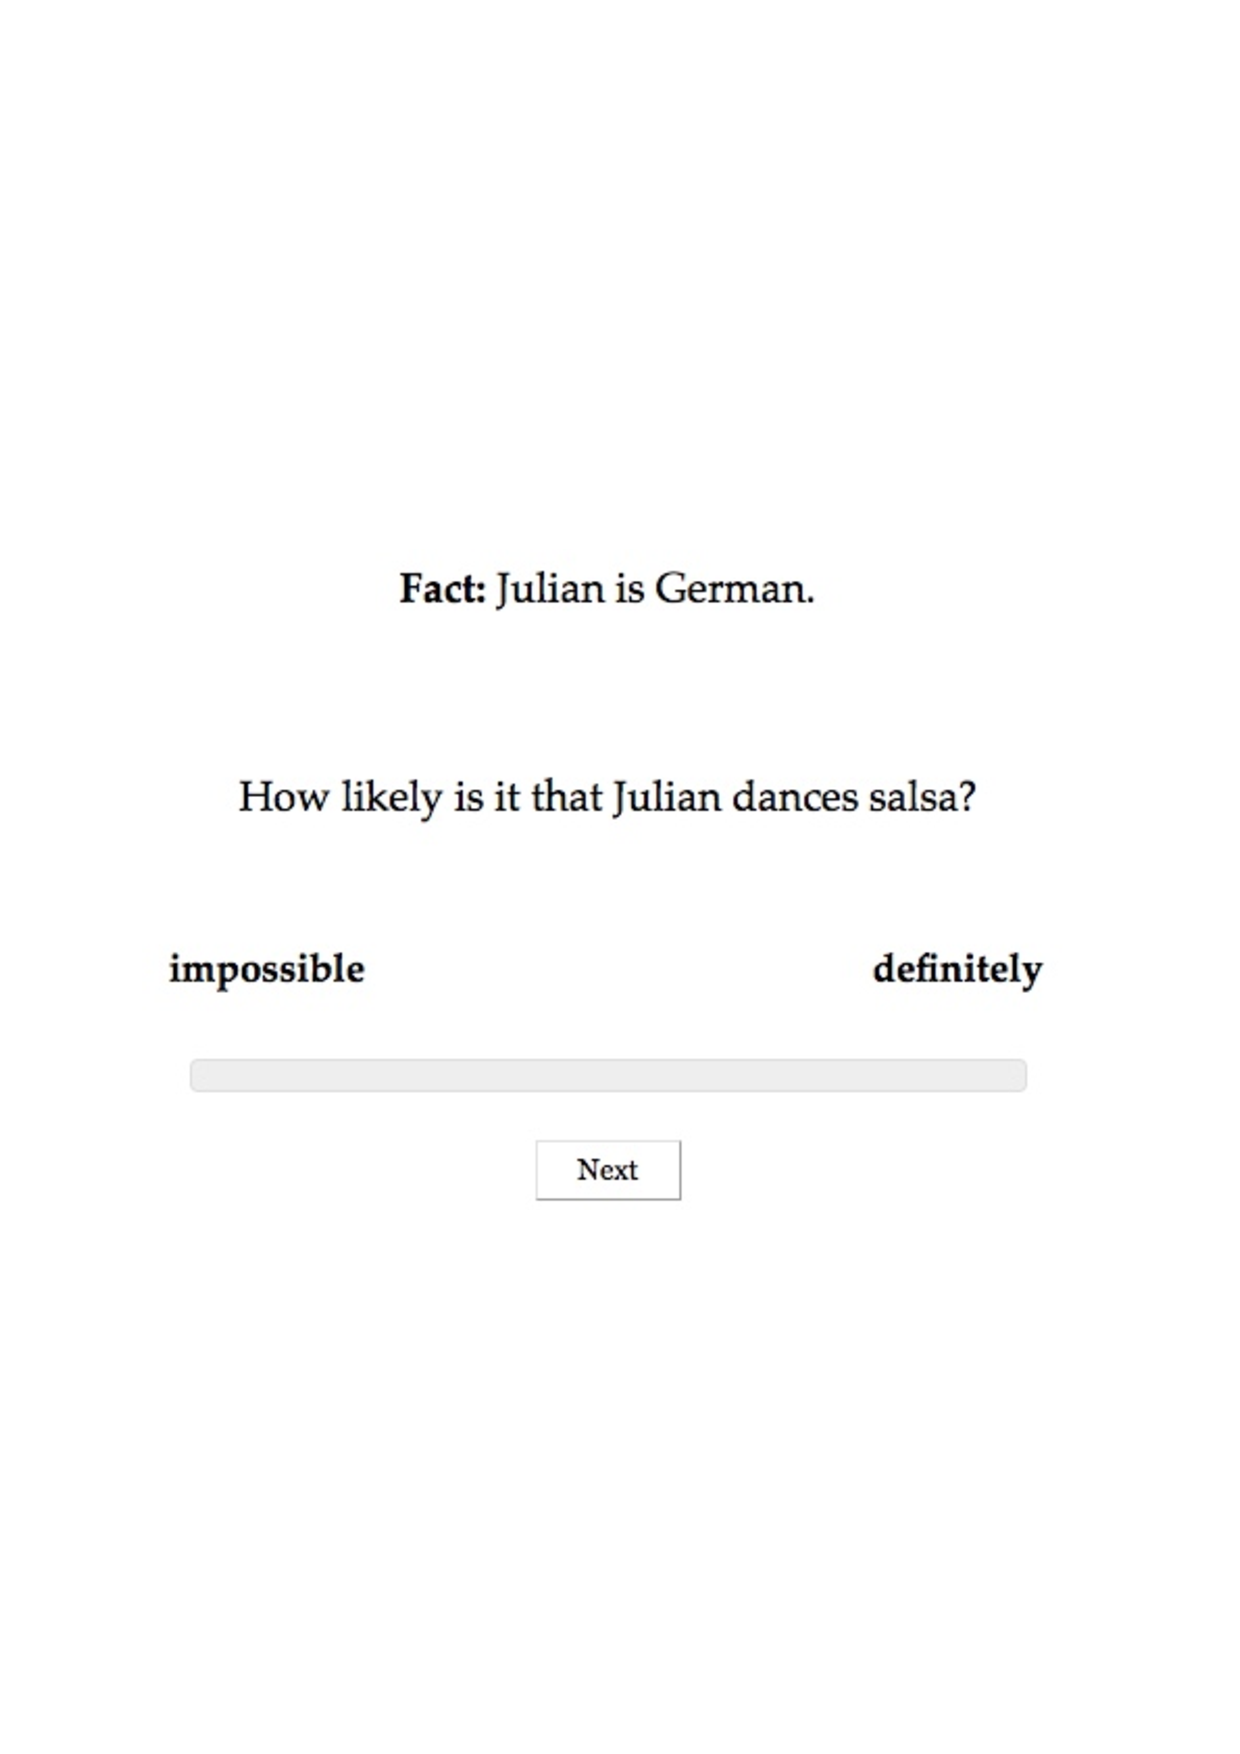
\includegraphics[width=7.55cm]{figures/exp1-prior-trial}}
%\caption{Target trial in prior block.}\label{fig-exp1-prior}
%\end{subfigure}%
%\begin{subfigure}[t]{0.5\textwidth}
%\centering
%\fbox{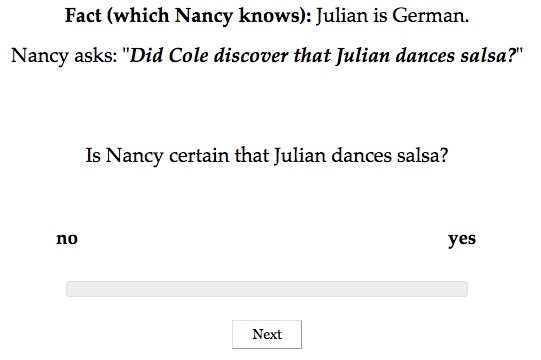
\includegraphics[width=7.9cm]{figures/exp1-projection-trial}} 
%\caption{Target trial in projection block.}\label{fig-exp1-projection}
% \end{subfigure}
% \par\bigskip
%\begin{subfigure}[t]{1\textwidth}
%        \centering
%       \fbox{\begin{minipage}{15cm}{\em acknowledge, admit, announce, be annoyed, be right, confess, confirm, demonstrate, discover, establish, hear, inform, know, pretend, prove, reveal, say, see, suggest, think. }\end{minipage}}
%\caption{20 clause-embedding predicates.}\label{fig-exp1-preds}
%\end{subfigure}
%\par\bigskip
%\begin{subfigure}[t]{0.5\textwidth}
%        \centering
%\fbox{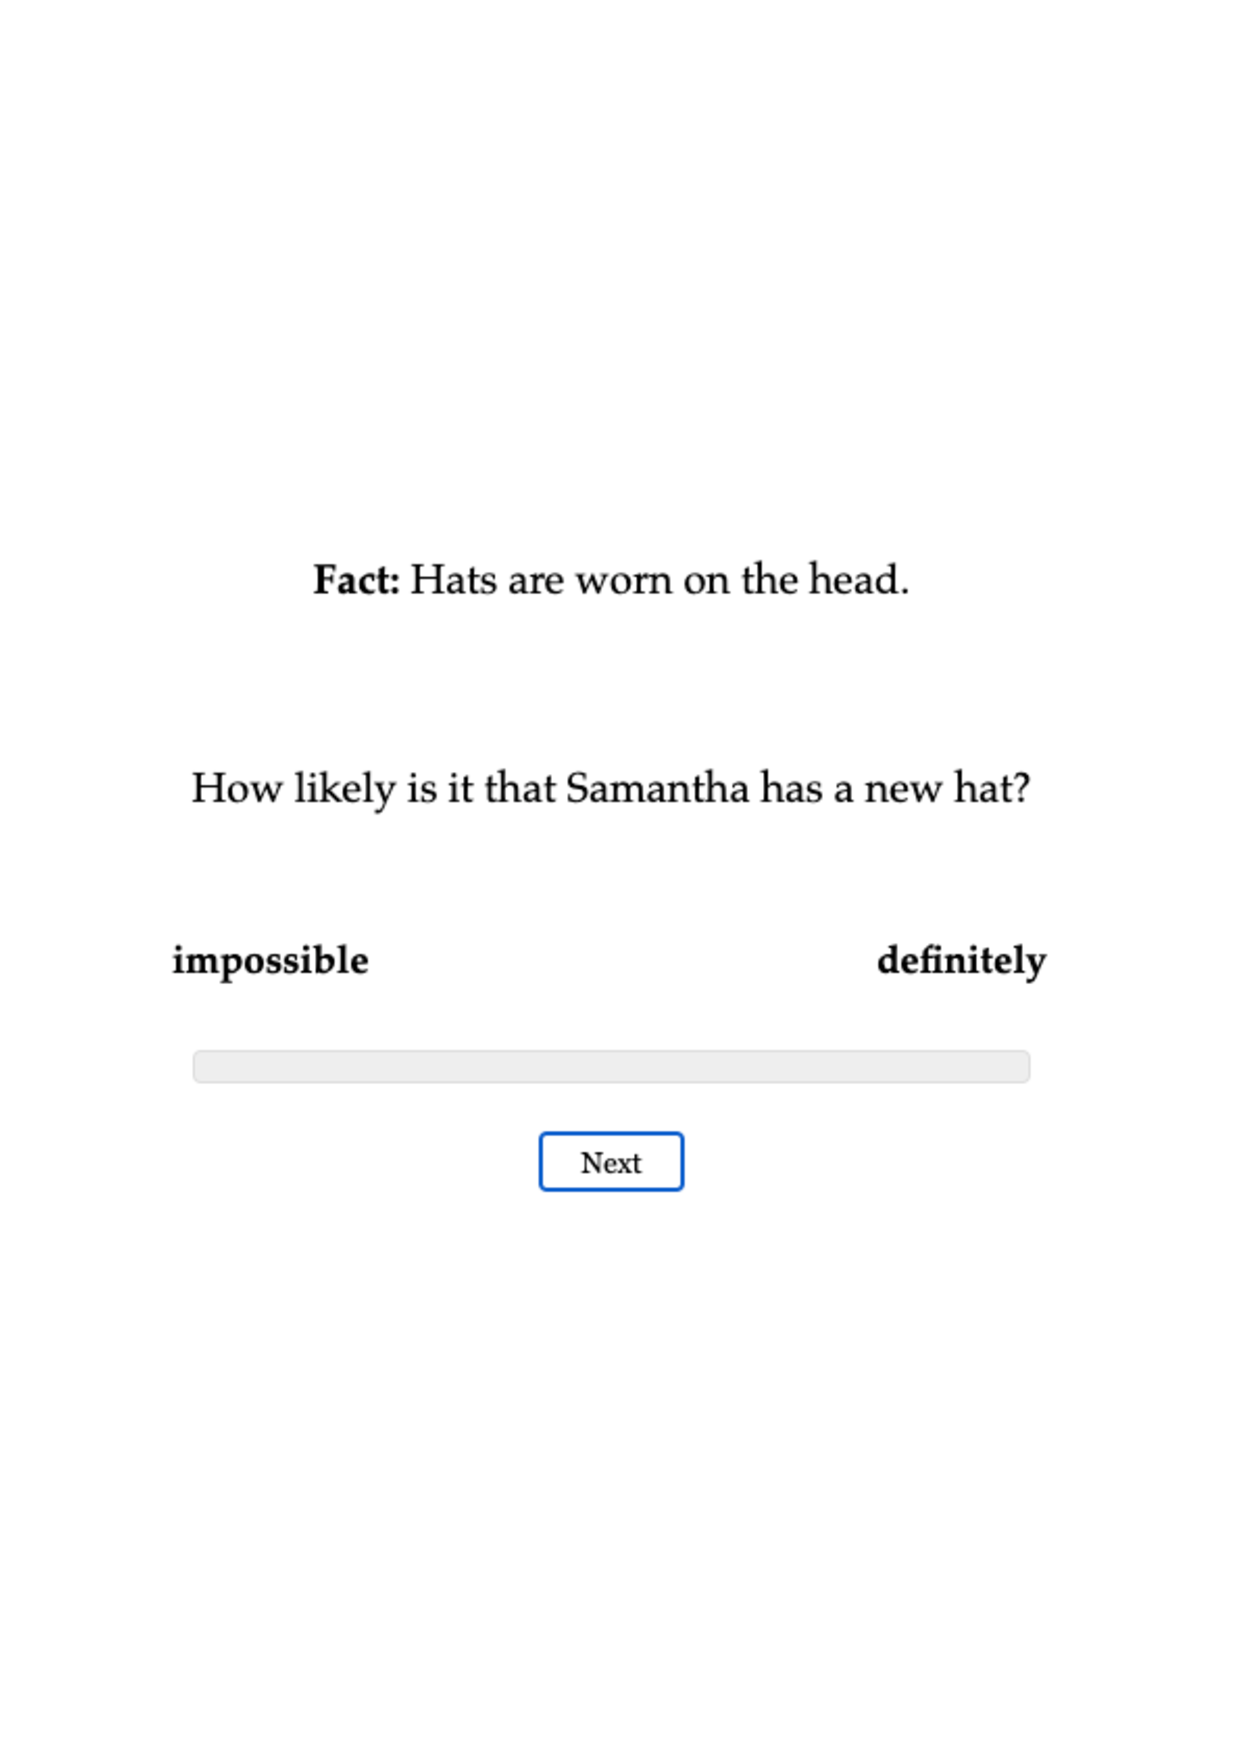
\includegraphics[height=5.4cm,width=7.6cm]{figures/exp1-prior-filler}}
%\caption{Filler trial in prior block.}\label{fig-exp1-prior-filler}
% \end{subfigure}%
%\begin{subfigure}[t]{0.5\textwidth}
%\centering
%\fbox{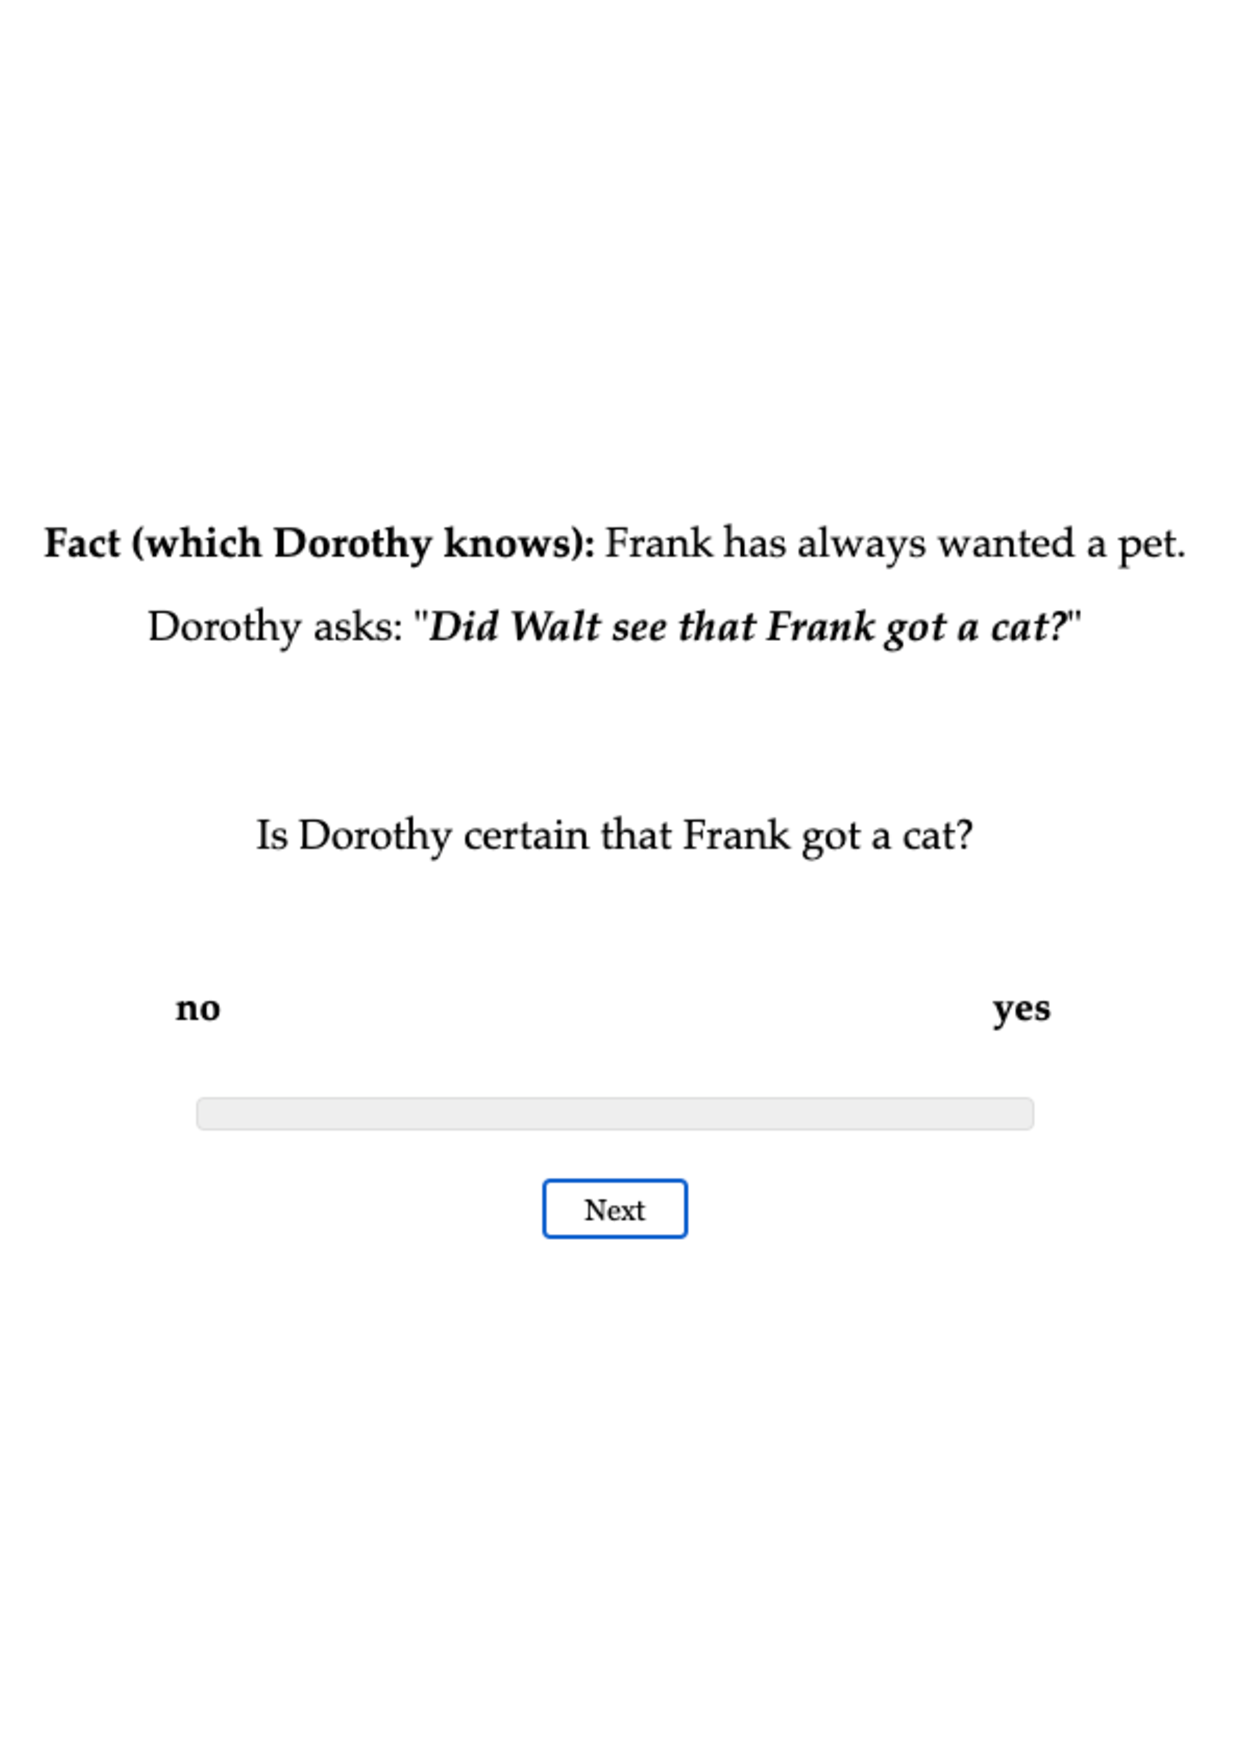
\includegraphics[height=5.4cm,width=7.9cm]{figures/exp1-projection-control}} 
%\caption{Control trial in projection block.}\label{fig-exp1-projection-control}
%\end{subfigure}
%
%
%\caption{Sample trials and 20 clause-embedding predicates in Exp.~1.}
%\end{figure}


\begin{figure}[h!]
\centering
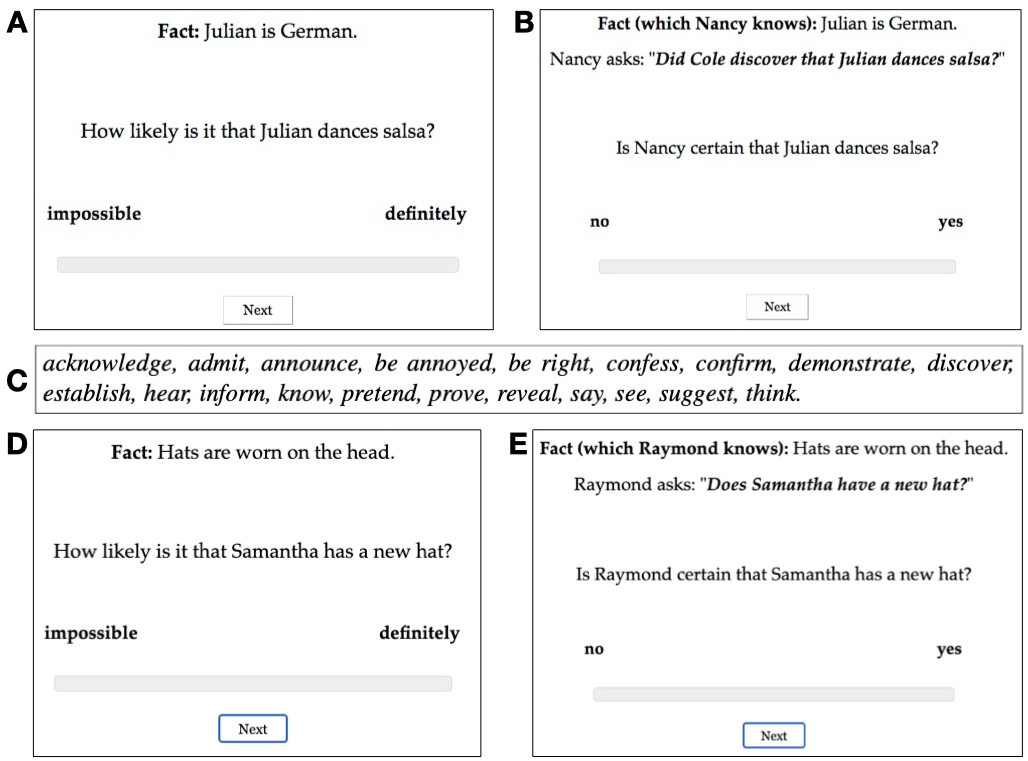
\includegraphics[width=\textwidth]{figures/complex-figure/complex-figure.jpeg}
\caption{\textbf{Example trials and 20 clause-embedding predicates.} \textbf{A}. Example target trial in prior block. \textbf{B}. Example target trial in projection block. \textbf{C}. The 20 clause-embedding predicates.  \textbf{D}. Example filler trial in prior block. \textbf{E}. Example control trial in projection block.}
\label{fig:fig-exp1}
\end{figure}

%\begin{exe}
%\ex\label{stim} 
%\begin{xlist}
%\ex {\bf Fact (which Carol knows):} Julian is Cuban.  \\ 
%{\bf Carol:} Does Sandra know that Julian dances salsa?
%\ex {\bf Fact (which Carol knows):} Julian is German.  \\ 
%{\bf Carol:} Does Sandra know that Julian dances salsa?
%\end{xlist}
%\end{exe}


%\begin{exe}
%\ex\label{target}  
%\begin{xlist}
%\ex {\bf Fact:} Julian is Cuban. \\ How likely is it that Julian dances salsa?
%\ex {\bf Fact:} Julian is German.  \\ How likely is it that Julian dances salsa?
%\end{xlist}
%\end{exe}

The projection block also included 6 control trials, which functioned as attention checks. The content of these stimuli was expected not to project: For example, in Figure \ref{fig:fig-exp1}D, the speaker is not committed to the main clause content, that Samantha has a new hat. The same 6 main clauses were also used to form 6 filler trials in the prior block; a sample stimulus is given in Figure \ref{fig:fig-exp1}E. These filler stimuli were not used to assess participants' attention. For the full set of stimuli see Supplementary Materials.


Each participant's stimulus set was semi-randomly generated by first randomly pairing up the 20 predicates and clauses. Half of the stimuli were then randomly assigned the respective clause's higher-probability fact, and half its lower-probability fact. Participants completed a total of 52 trials: 20 target trials in each block, 6 control trials in the projection block, and 6 filler trials in the prior block. Each participant completed the same 6 filler and control trials. Block order and within-block trial order were randomized.



After completing the experiment, participants filled out a short optional demographic survey. To encourage truthful responses, participants were told that they would be paid no matter what answers they gave in the survey.

\paragraph{Data exclusion} Data was excluded based on self-declared non-native speaker status and other criteria given in the Supplementary Materials, leaving 5,720 data points from 286 participants to be analyzed (ages 18-82; median: 35.5; 116 female, 186 male, 1 other, 1 undeclared).

\subsection{Results and discussion}

\paragraph{Prior beliefs.}  Figure \ref{f-prior} shows the mean prior probabilities of the 20 contents by fact. We conducted a  mixed-effects linear regression predicting slider rating from dummy-coded fact type (reference level: `lower probability') and random by-item and by-participant intercepts and slopes for fact type.\footnote{All analyses were conducted in R \citep{R} using the \texttt{lme4} package \citep{lme4}.} Each content's mean prior probability  was rated as higher when it was presented with its higher probability fact than when it was presented with its lower probability fact ($\beta$ = 0.45, $SE$ = 0.01, $t$ = 31.12, $p$ $<$ .0001). This suggests that the manipulation of the prior probability of the 20 contents was successful. 

\begin{figure}[h!]
\centering
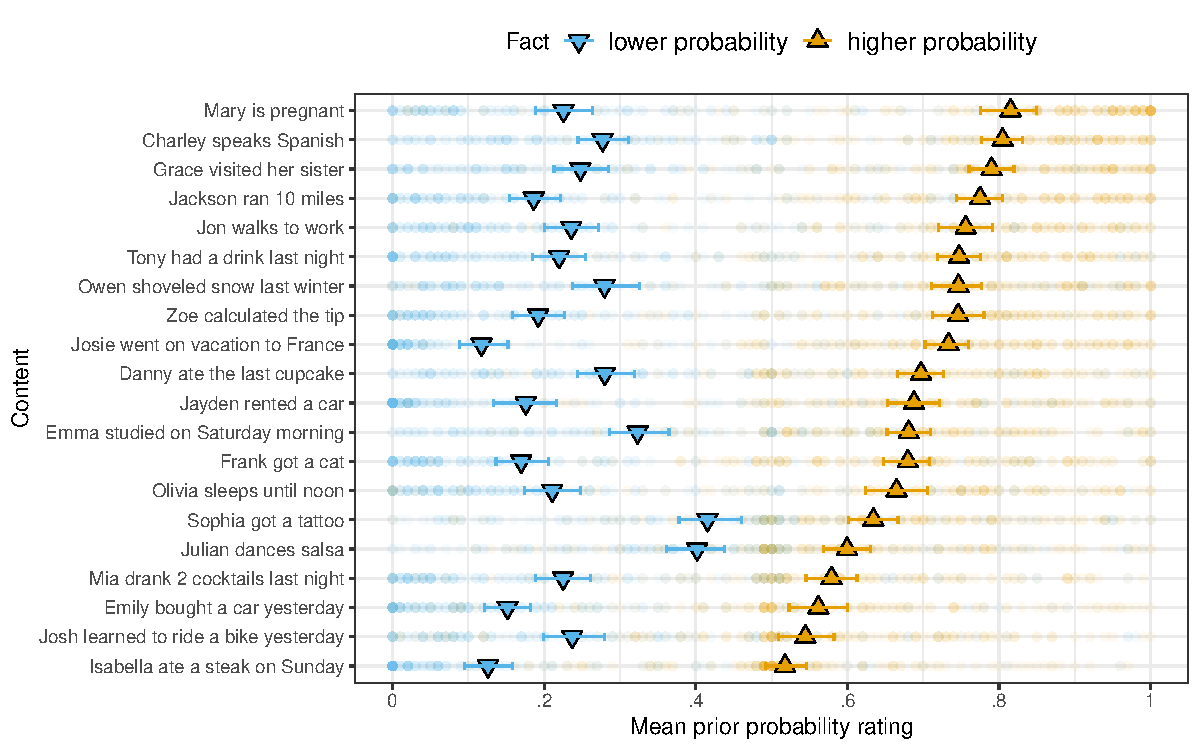
\includegraphics[width=\textwidth]{../../results/9-prior-projection/graphs/prior-ratings}

\caption{Mean prior probability by content and fact in Exp.~1. Error bars indicate 95\% bootstrapped confidence intervals. Transparent dots indicate individual participant ratings.} 
\label{f-prior}
\end{figure}

\paragraph{Do prior beliefs modulate projection?}  Figure \ref{f-projection-mean} shows the mean certainty ratings for the CCs by  predicate and by fact, as well as the mean certainty rating for the main clause controls (abbreviated `MC'). We conducted a mixed effects linear regression predicting certainty ratings from dummy-coded fact type (reference level: `lower probability') and random by-item and by-participant intercepts and slopes for fact type. The mean certainty ratings were higher for contents  presented with higher probability facts than for contents presented with lower probability facts ($\beta$ = 0.14, $SE$ = 0.01, $t$ = 12.24, $p$ $<$ .0001).   The same was true when using the group-level by-item mean prior belief as a predictor  ($\beta$ = 0.31, $SE$ = 0.02, $t$ = 12.58, $p$ $<$ .0001).   This suggests that participants' prior beliefs about content probability systematically modulated the extent to which they take the speaker to be committed to that content.

\begin{figure}[h!]
\centering

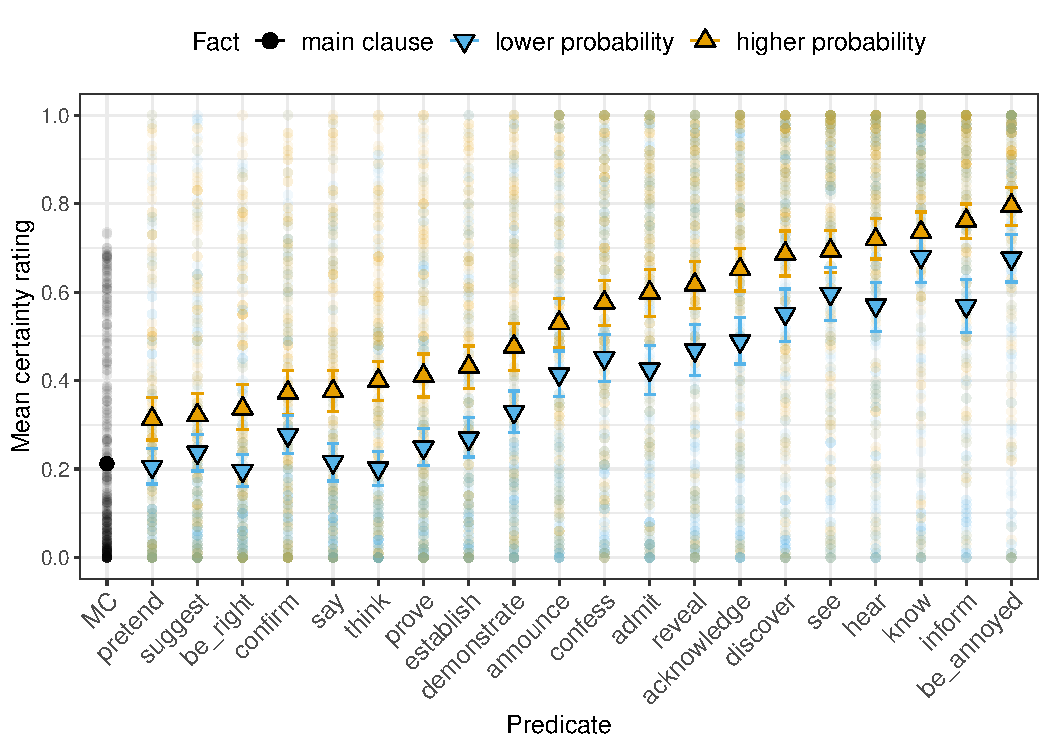
\includegraphics[width=\textwidth]{../../results/9-prior-projection/graphs/means-projectivity-by-predicate-and-prior}

\caption{Mean certainty ratings by predicate and prior probability of the content of the complement in Exp.~1. Error bars indicate 95\% bootstrapped confidence intervals. Light dots indicate participants' ratings.} 
\label{f-projection-mean}
\end{figure}

We also replicated the by-predicate variability in the projection of the CC observed by \citep{tonhauser-degen-factive}: for instance, the CC of {\em be annoyed} was more projective than that of {\em discover}, which in turn was more projective than that of {\em announce}. The Spearman rank correlation between the mean certainty ratings in Exp.~1 (collapsing over facts) and Exp.~1a of \citep{tonhauser-degen-factive} is  .991; see Supplementary Materials for a visualization. Exp.~1 thereby also provides further evidence for the systematic influence of the predicate on projection. Crucially, the effect of the prior was observable independently of predicate.

\begin{figure}[h!]
%\centering

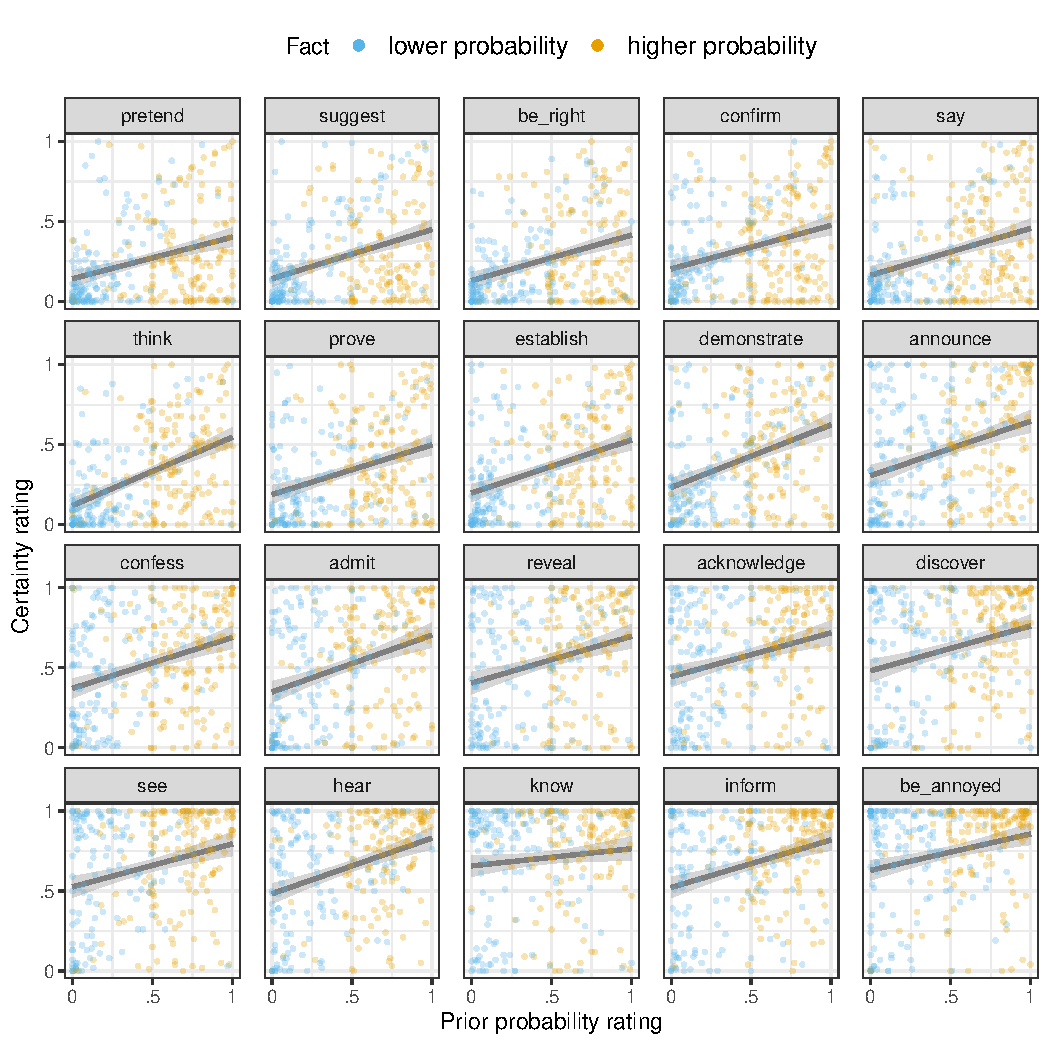
\includegraphics[width=\textwidth]{../../results/9-prior-projection/graphs/projection-by-prior}

\caption{Certainty ratings against individual prior probability ratings for each predicate in Exp.~1. Linear smoothers with 95\% confidence intervals are overlaid.}
\label{f-projection}
\end{figure}


Closer inspection of  Figure \ref{f-prior} reveals by-participant variability in prior probability ratings, suggesting that individual participants' prior beliefs may not align with the prior probability classification assumed in  Figure \ref{f-projection-mean}. For example, given a particular content ({\em Julian dances salsa}), it is possible that one participant's prior probability rating was lower than that of another participant, even though the first participant was presented with the higher probability fact ({\em Julian is Cuban}) and the second one with the lower probability fact ({\em Julian is German}). Figure \ref{f-projection} shows participants' certainty ratings by their individual prior probability ratings. %(The color coding here merely represents the type of fact the participant was presented with. No classification is imposed.) The linear smoothers suggest a positive correlation for each predicate between prior probability and certainty ratings such that contents with higher prior probability ratings receive higher certainty ratings. 
To investigate whether prior beliefs modulate projection at the by-participant level,  we conducted the same mixed-effects analysis reported above, but used participants' individual, continuous prior probability ratings as the fixed effect prior predictor. Again, higher-prior-probability CCs were more likely to project ($\beta$ = 0.28, $SE$ = 0.02, $t$ = 13.85, $p$ $<$ .0001). This  suggests that prior beliefs modulate projection even at the by-participant level. In fact, a Bayesian Information Criterion (BIC) model comparison  revealed that the individual-level model better captured the variance in the data (categorical model BIC: 2654; group-level model BIC: 2586; individual-level model BIC: 2291),\footnote{The BIC model comparisons were not pre-registered, so we also ran AIC model comparisons as a robustness check. The results were qualitatively identical (categorical model AIC: 2607; group-level model AIC: 2539; individual-level model AIC: 2244).} suggesting that individual listeners' prior beliefs systematically modulate the extent to which they take the speaker to be committed to a content: the more they believe it, the more they take the speaker to believe it.


%\newpage
%
%The qualitative observations about the relations between prior probability, clause-embedding predicate and projection were borne out statistically. We fitted a Bayesian mixed effects Beta regression model  with weakly informative priors using the \verb|brms| \citep{buerkner2017}  package in R \citep{R} on the target data (5,720 data points). The model predicted the certainty ratings from a fixed effect of prior probability and included the maximal random effects structure justified by the design, namely random by-participant and by-item intercepts (where an item is a combination of a predicate and a complement clause). A Beta regression model estimates the mean of the outcome distribution (like a linear regression model).\footnote{Beta regression models also estimate a second parameter, namely the precision, which is a measure of dispersion: the greater the precision, the more concentrated the ratings are around the mean. In this paper, we rely on the estimated mean to identify whether prior probability predicts projection. Both the estimated mean and precision are reported in the full model output table in Supplement \ref{modeldetails}.} We thus obtain a 95\% credible interval for \jt{the mean effect of prior probability on certainty?}. Supplement \ref{modeldetails} motivates the use of Beta regression over linear regression, provides a brief primer on how to interpret Bayesian mixed effects Beta regression models, and reports the full model output.
%
%\jt{We need to report two models here: predicting projection from prior at by-participant level, but also predicting mean projection from mean prior, to allow for comparison to Exps.~2}
%
%\jt{According to the Beta regression model, the estimated mean for each predicate was higher when....} 


The results of Exp.~1 provide empirical support for the hypothesis that higher prior probability content is more likely to project. It is possible, however, that the within-participant design resulted in participants' responses on either block influencing their responses on the other block. To guard against this possibility, we replicated Exp.~1 by collecting prior probability and projection ratings from different groups.  

\section{Experiment 2}\label{s3}

Exps.~2a and 2b measured the prior probability and the projection of the 20 contents of Exp.~1, respectively.

\subsection{Methods}

%Exp 2a: November 13, 2017
%Exp 2b: November 28, 2017

\paragraph{Participants} Participants with U.S.\ IP addresses and at least 99\% of previous HITs approved were recruited on Amazon's Mechanical Turk platform. The 95 participants in Exp.~2a (ages: 21-75, median: 33; 45 female, 50 male) were paid 55 cents. The 300 participants in Exp.~2b (ages: 21-72, median: 36; 145 female, 154 male, 1 undeclared) were paid 85 cents.

\paragraph{Materials and procedures} The target stimuli of Exp.~2a were identical to those of the prior block of Exp.~1. Each participant saw two control stimuli as attention checks (see Supplementary Materials). The materials of Exp.~2b were identical to those of the projection block of Exp.~1. Trial order in both experiments was random. The procedures of Exps.~2a and 2b were identical to those of the prior and projection blocks of Exp.~1, respectively.

\paragraph{Data exclusion} We excluded data based on the criteria given in the Supplementary Materials, leaving data from 75 participants to be analyzed in Exp.~2a (1,500 data points; ages 21-75; median: 35; 34 female, 41 male) and from 266 participants in Exp.~2b (5,320 data points; ages 21-72; median: 36; 129 female, 136 male, 1 undeclared).

\subsection{Results and discussion}

\paragraph{Prior beliefs.} Exp.~2a successfully replicated the prior probability manipulation of Exp.~1: contents were rated as more likely when presented with a higher probability fact ($\beta$ = 0.54, $SE$ = 0.04, $t$ = 15.07, $p$ $<$ .0001).  Figure \ref{f-prior-comparison} shows contents' mean prior probability ratings in Exp.~2a against those of Exp.~1. The Spearman rank correlation was very high, at $r=$.977. For a visualization of the by-content prior ratings see Supplementary Materials.

\begin{figure}[h!]

\centerline{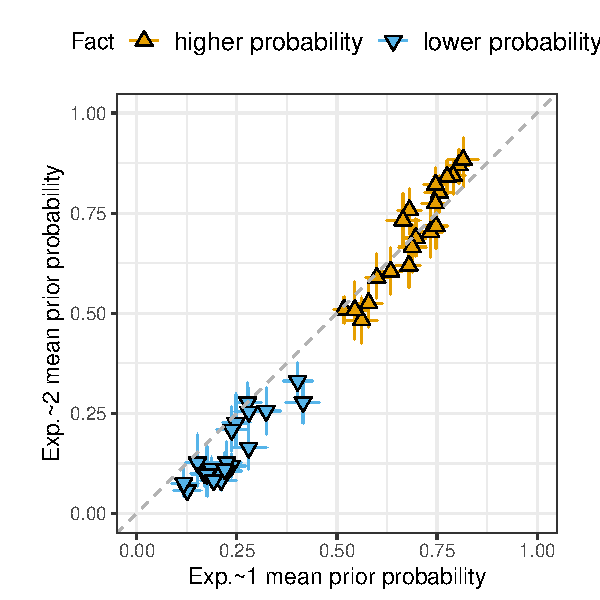
\includegraphics[width=.4\paperwidth]{../../results/1-prior/graphs/prior-probability-comparison-exp1-exp2}}

\caption{Mean prior probability ratings in Exp.~2a against those of Exp.~1. Error bars indicate 95\% bootstrapped confidence intervals.}
\label{f-prior-comparison}
\end{figure}


\paragraph{Do prior beliefs modulate projection?} Mean certainty ratings were higher for contents  presented with higher prior probability facts than for contents presented with lower prior probability facts (see Figure \ref{f-projection-mean-2b}). This was true when the prior predictor was entered as a categorical predictor (reference level: `lower probability'; $\beta$ = 0.18, $SE$ = 0.01, $t$ = 12.81, $p$ $<$ .0001) and when it was entered as a continuous predictor representing group-level prior means ($\beta$ = 0.34, $SE$ = 0.03, $t$ = 13.27, $p$ $<$ .0001). Thus, Exp.~2b replicates the critical result of Exp.~1 that prior content probability modulates its projection.\footnote{28 participants took Exp.~2b after taking Exp.~2a two weeks before. Analyses that excluded these participants' data did not change the results. Exp.~2b also replicated \citep{tonhauser-degen-factive}'s result that there is by-predicate variability in the projection of the CC; see Supplementary Materials.}  The replication suggests that the result of Exp.~1 is not an artifact of the within-participant design of Exp.~1.

\begin{figure}[h!]
\centering

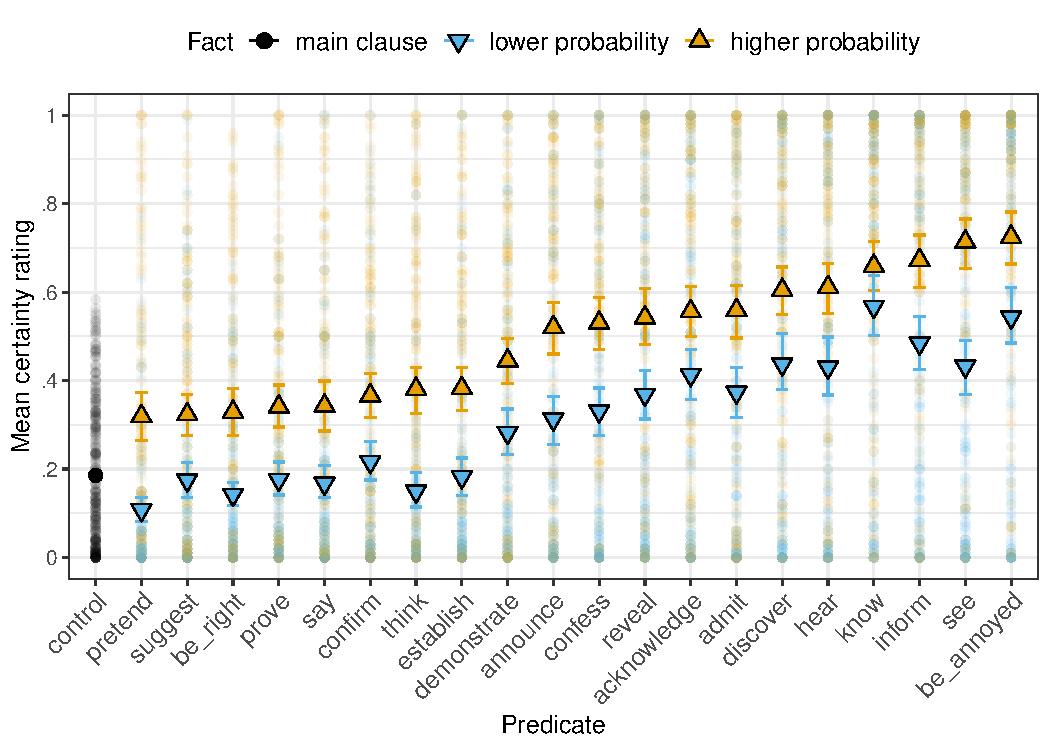
\includegraphics[width=\textwidth]{../../results/3-projectivity/graphs/means-projectivity-by-predicate-and-prior}

\caption{Mean certainty ratings by predicate and prior probability of the content of the complement in Exp.~2b. Error bars indicate 95\% bootstrapped confidence intervals. Light dots indicate participants' ratings.} 
\label{f-projection-mean-2b}
\end{figure}

\section{General discussion and concluding remarks}
\label{s4}


We tested whether listeners' prior beliefs modulate projection. While previous research on this question has yielded conflicting results \citep{mahler2020, lorson2018}, we showed in two experiments that content is more likely to project the more a priori likely it is, thus confirming \citet{mahler2020}'s ({\bf JT: PROBLEMATIC!!}) results and expanding on them in several ways. First, while \citet{mahler2020} manipulated only the political party affiliation of the speaker, the manipulation in Exps.~1 and 2 relied on 20 distinct properties of individuals (e.g., whether Julian is more likely to dance salsa if he is German or Cuban). Thus, the results of Exps.~1 and 2 suggest a general effect of prior beliefs on projection. Second, our experiments show that prior beliefs modulate projection for a wider cross-section of clause-embedding predicates, including cognitive (e.g., {\em know}), emotive (e.g., {\em be annoyed}), communication (e.g., {\em announce}), and inferential (e.g., {\em prove}) predicates. Finally, the within-participant design of Exp.~1 shows that individuals' prior beliefs better predict projection than group-level beliefs, which in turn better predict projection than the binary categorical beliefs that \citet{mahler2020} investigated. This suggests that at least some by-participant variability observed in previous projection experiments  \citep[see, e.g.,][]{tbd-variability,tonhauser-degen-factive} may be due to participants assigning different prior probabilities to investigated content.

Our results have two broader implications. First, they suggest that the purview of projection analyses is wider than assumed by current analyses, which typically limit their attention to a narrow subset of clause-embedding predicates, like factive ones \citep[e.g.,][]{heim83,vds92,abrusan2011,abrusan2016,romoli2015,best-question}. Second, they motivate the development of projection analyses that consider listeners' variable subjective beliefs about the world. Given the gradient nature of the measured (prior and posterior) beliefs and the uncertainty inherent in the different factors that have been shown to modulate projection (e.g., at-issueness, prosody), probability theory suggests itself as a representational framework within which to model projection. To date, only few probabilistic models of  projection have been developed \citep{qing2016, stevens-etal2017}. In these models, projection is the result of listeners' reasoning about the common ground that the speaker is assuming and the likely question that was being addressed, respectively. While neither investigated the effect of prior beliefs explicitly, both models are couched within the Rational Speech Act (RSA) framework \citep{frankejaeger2016,GoodmanFrank2016}, which standardly assumes that utterance interpretation is modulated by listeners' prior beliefs. The RSA framework is thus equipped to capture the effects reported here. We see the implementation of projection analyses within RSA as a promising avenue for formalizing the intricate interplay of semantic and pragmatic factors in the projection of contents of complements of clause-embedding predicates, including the conventional contribution of predicates, content at-issueness, and subjective prior beliefs about content.



\acknowledgments
\jd{Enter your acknowledgments here.}

\section{Funding information}

\jd{jt enter info}
%% ie.,

% The authors thank Laurence Aitchison for fruitful discussions.  RKN
% and PD received funding from the Gatsby Charitable Foundation. Y-AB,
% RBS, KC and PS received funding from Canadian Institutes of Health
% Research grant $MOP74577$,
% Fond de recherche Qu\'{e}bec - Sant\'{e} (Group grant to the Groupe 
% de recherche en neurobiologie comportementale, Shimon Amir, P.I.), and
% Concordia University Research Chair (Tier I). 

\authorcontributions 
\jd{Who helped formulate the project, who supplied data, analyses and
experiments, etc.}

%% ie.
%% Project was formulated by RKN, PD, PS,
%% based on substantial data, analyses and experiments of Y-AB, KC, RS,
%% PS. RKN, PD formalised the model, RKN implemented and ran the model;
%% RKN analysed the molecular ethogram data; Y-AB formalised and
%% implemented a CTMC model. All authors wrote the manuscript.


%%%%%%%%%%%%%%%%%%%%%%%
%% The bibliography

%% The bibliography is made using only the entries that you cite using 
%% \citep{}, or one of the Natbib citation entries, like \citep{}, \citet{} etc.

\bibliography{../../bibliography}

%ie.,
%\bibliography{bibsamp}

%% Optional Appendix
%\appendix

%\section{Sample Appendix Section}


\end{document}




\section{Sample citations}
For general information on the correct form for citations using
the APA 6 format, see the following sites:
\href{https://owl.english.purdue.edu/owl/resource/560/02/}
{APA 6, In-text citations, The Basics} and
\href{https://owl.english.purdue.edu/owl/resource/560/03/}
{APA 6, In-text citations}

\section{Natbib citation mark up}

\subsection{Single citations}
\noindent
\begin{tabular}{ll}
\bf Type&\bf Results\\
\hline
\verb+\citet{jon90}+&Jones et al. (1990)\\
\verb+\citet[chap. 2]{jon90}+&Jones et al. (1990, chap. 2)\\
    \verb+\citep{jon90}+	    &   	(Jones et al., 1990)\\
    \verb+\citep[chap. 2]{jon90}+ 	&    	(Jones et al., 1990, chap. 2)\\
    \verb+\citep[see][]{jon90}+ 	 &    	(see Jones et al., 1990)\\
    \verb+\citep[see][chap. 2]{jon90}+ 	&    	(see Jones et al., 1990, chap. 2)\\
    \verb+\citet*{jon90}+ 	    &    	Jones, Baker, and Williams (1990)\\
    \verb+\citep*{jon90}+	    &    	(Jones, Baker, and Williams,
    1990) \\
\end{tabular}

For example, some citations from the OpenMindSample bibliography:
citet:\citet{anderson}, citep:\citep{antibayes}, and
cite*: \citet*{anderson}.

\subsection{Multiple citations}
Multiple citations may be made by including more than one citation
key in the \verb+\cite+ command argument.

\noindent
\begin{tabular}{ll}
\bf Type&\bf Results\\
\hline
\verb+\citet{jon90,jam91}+&Jones et al. (1990); James et al. (1991)\\
\verb+\citep{jon90,jam91}+&(Jones et al., 1990; James et al. 1991)\\
\verb+\citep{jon90,jon91}+&(Jones et al., 1990, 1991)\\
\verb+\citep{jon90a,jon90b}+&(Jones et al., 1990a,b)\\
\end{tabular}

For example, multiple citations from the OpenMindSample bibliography:
citet:\citet{anderson,antibayes}, citep:\citep{anderson,antibayes}.
As you see, the citations are automatically hyperlinked to their
reference in the bibliography.

\newpage

\section{Sample figures}

\begin{figure}[h] 
\centerline{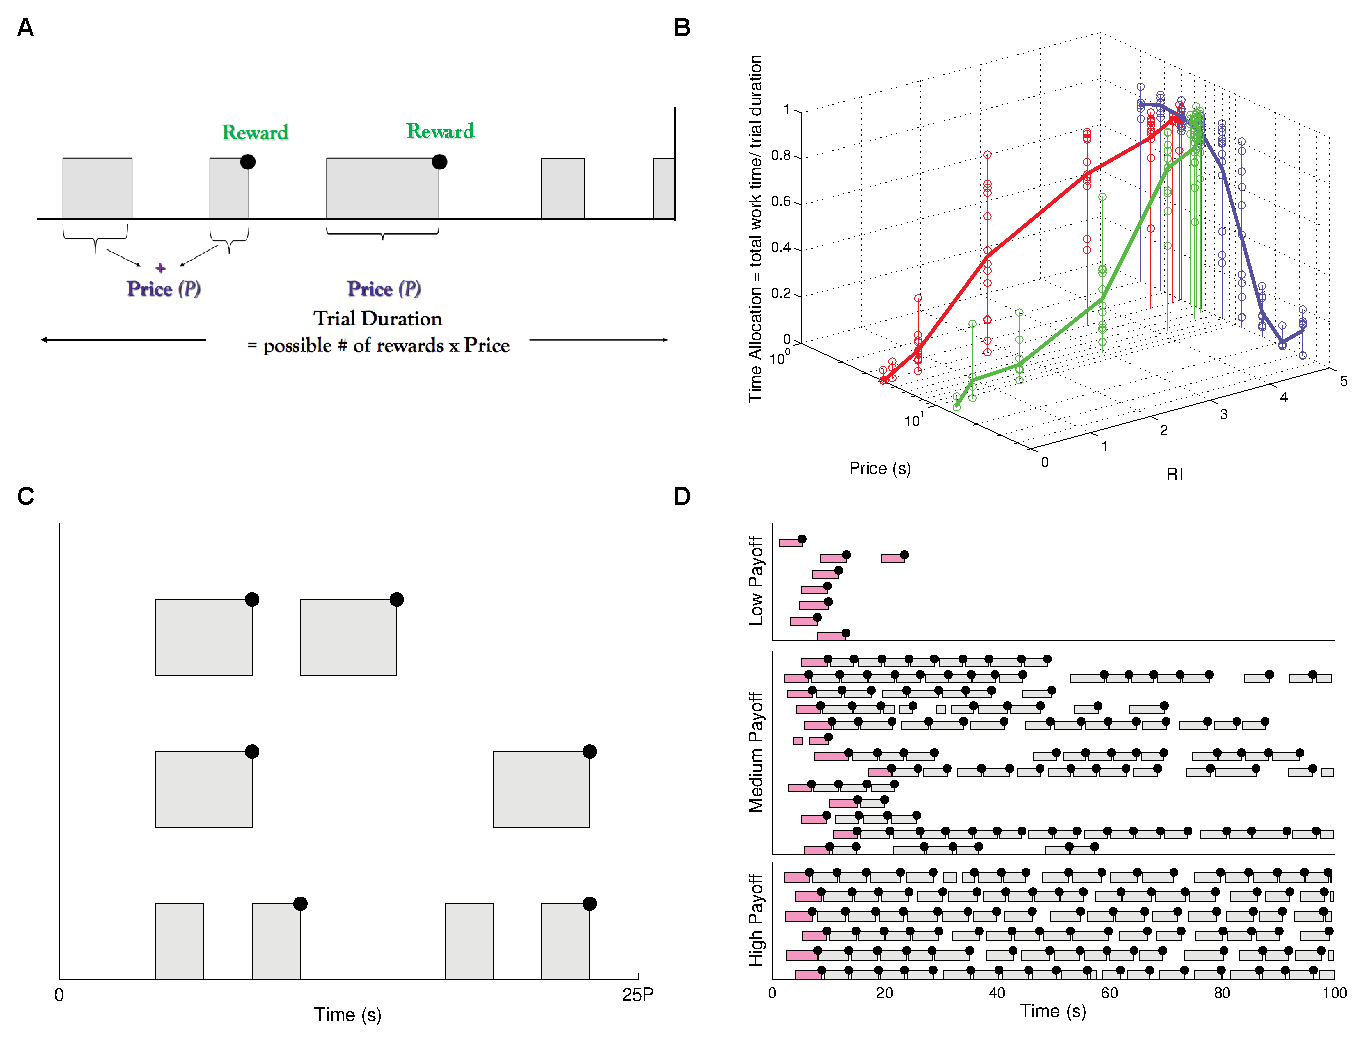
\includegraphics[width=\textwidth]{Fig1}}
\caption{(Colour online) \textbf{Task and key features of the
 data.} \\
 A) Cumulative handling time (CHT) task. Grey bars denote work
(depressing a lever), white gaps show leisure. The subject must
 accumulate work up to a total period of time called the
\emph{price} ($P$) in order to obtain a single reward (black dot) of subjective reward
intensity $RI$. The trial duration is $25\times \mathrm{price}$ (plus
$2$s each time the price is attained, during which the lever is retracted so it cannot
work; not shown).
}
\label{fig:task_data}
\end{figure}

\begin{figure}[ht] 
\widefigure{\fullpagewidth}{Fig1}
\caption{(Colour online) \textbf{Task and key features of the
 data.} \\
A) Cumulative handling time (CHT) task. Grey bars denote work
(depressing a lever), white gaps show leisure. The subject must
accumulate work up to a total period of time called the
\emph{price} ($P$) in order to obtain a single reward (black dot) of subjective reward
intensity $RI$. The trial duration is $25\times \mathrm{price}$ (plus
$2$s each time the price is attained, during which the lever is retracted so it cannot
work; not shown).
}
\label{newfig:task_data}
\end{figure}

\clearpage
\section{Sample tables}

\begin{table}[!ht]
\caption{Time of the Transition Between Phase 1 and Phase 2$^{a}$}
\label{tab:label}
\centering
\begin{tabular}{lc}
\hline
 Run  & Time (min)  \\
\hline
  $l1$  & 260   \\
  $l2$  & 300   \\
  $l3$  & 340   \\
  $h1$  & 270   \\
  $h2$  & 250   \\
  $h3$  & 380   \\
  $r1$  & 370   \\
  $r2$  & 390   \\
\hline
\multicolumn{2}{l}{$^{a}$Table note text here.}
\end{tabular}
\end{table}

\begin{table}[ht]
\widecaption{Sample table taken from [treu03]\label{tbl-1}}
\begin{widetable}
\advance\tabcolsep-1pt
\small
\begin{tabular}{ccrrccccccccc}
\hline
\bf 
POS &\bf  chip &\multicolumn1c{\bf ID} &\multicolumn1c{\bf X}
&\multicolumn1c{\bf Y} &\bf
RA &\bf DEC &\bf IAU$\pm$ $\delta$ IAU &\bf
IAP1$\pm$ $\delta$ IAP1 &\bf IAP2 $\pm$ $\delta$
IAP2 &\bf star &\bf E &\bf Comment\\
\hline
0 & 2 & 1 & 1370.99 & 57.35\rlap{$^a$}    &   6.651120 &  17.131149 &
21.344$\pm$0.006\rlap{$^b$}  & 2 4.385$\pm$0.016 & 23.528$\pm$0.013 & 0.0 & 9 & -    \\
0 & 2 & 2 & 1476.62 & 8.03     &   6.651480 &  17.129572 & 21.641$\pm$0.005  & 2 3.141$\pm$0.007 & 22.007$\pm$0.004 & 0.0 & 9 & -    \\
0 & 2 & 3 & 1079.62 & 28.92    &   6.652430 &  17.135000 & 23.953$\pm$0.030  & 2 4.890$\pm$0.023 & 24.240$\pm$0.023 & 0.0 & - & -    \\
0 & 2 & 4 & 114.58  & 21.22    &   6.655560 &  17.148020 & 23.801$\pm$0.025  & 2 5.039$\pm$0.026 & 24.112$\pm$0.021 & 0.0 & - & -    \\
0 & 2 & 5 & 46.78   & 19.46    &   6.655800 &  17.148932 & 23.012$\pm$0.012  & 2 3.924$\pm$0.012 & 23.282$\pm$0.011 & 0.0 & - & -    \\
0 & 2 & 6 & 1441.84 & 16.16    &   6.651480 &  17.130072 & 24.393$\pm$0.045  & 2 6.099$\pm$0.062 & 25.119$\pm$0.049 & 0.0 & - & -    \\
0 & 2 & 7 & 205.43  & 3.96     &   6.655520 &  17.146742 & 24.424$\pm$0.032  & 2 5.028$\pm$0.025 & 24.597$\pm$0.027 & 0.0 & - & -    \\
0 & 2 & 8 & 1321.63 & 9.76     &   6.651950 &  17.131672 &
22.189$\pm$0.011  & 2 4.743$\pm$0.021 & 23.298$\pm$0.011 & 0.0 & 4 &
edge \\
\hline
\multicolumn{13}{l}{%
Table 2 is published in its entirety in the electronic
edition of the {\it Astrophysical Journal}.}\\[3pt]
\multicolumn{13}{l}{%
$^a$ Sample footnote for table 2.}\\[3pt]
\multicolumn{13}{l}{%
$^b$ Another sample footnote for table 2.}
\end{tabular}
\end{widetable}
\end{table}

\begin{table}[p]
\rotatebox{90}{\vbox{\hsize=\textheight
\caption{Here is a caption for a table that is found in landscape
mode.}
\begin{tabular}{ccrrccccccccc}
\hline
\bf 
POS &\bf  chip &\multicolumn1c{\bf ID} &\multicolumn1c{\bf X}
&\multicolumn1c{\bf Y} &\bf
RA &\bf DEC &\bf IAU$\pm$ $\delta$ IAU &\bf
IAP1$\pm$ $\delta$ IAP1 &\bf IAP2 $\pm$ $\delta$
IAP2 &\bf star &\bf E &\bf Comment\\
\hline
0 & 2 & 1 & 1370.99 & 57.35\rlap{$^a$}    &   6.651120 &  17.131149 &
21.344$\pm$0.006\rlap{$^b$}  & 2 4.385$\pm$0.016 & 23.528$\pm$0.013 & 0.0 & 9 & -    \\
0 & 2 & 2 & 1476.62 & 8.03     &   6.651480 &  17.129572 & 21.641$\pm$0.005  & 2 3.141$\pm$0.007 & 22.007$\pm$0.004 & 0.0 & 9 & -    \\
0 & 2 & 3 & 1079.62 & 28.92    &   6.652430 &  17.135000 & 23.953$\pm$0.030  & 2 4.890$\pm$0.023 & 24.240$\pm$0.023 & 0.0 & - & -    \\
0 & 2 & 4 & 114.58  & 21.22    &   6.655560 &  17.148020 & 23.801$\pm$0.025  & 2 5.039$\pm$0.026 & 24.112$\pm$0.021 & 0.0 & - & -    \\
0 & 2 & 5 & 46.78   & 19.46    &   6.655800 &  17.148932 & 23.012$\pm$0.012  & 2 3.924$\pm$0.012 & 23.282$\pm$0.011 & 0.0 & - & -    \\
0 & 2 & 6 & 1441.84 & 16.16    &   6.651480 &  17.130072 & 24.393$\pm$0.045  & 2 6.099$\pm$0.062 & 25.119$\pm$0.049 & 0.0 & - & -    \\
0 & 2 & 7 & 205.43  & 3.96     &   6.655520 &  17.146742 & 24.424$\pm$0.032  & 2 5.028$\pm$0.025 & 24.597$\pm$0.027 & 0.0 & - & -    \\
0 & 2 & 8 & 1321.63 & 9.76     &   6.651950 &  17.131672 &
22.189$\pm$0.011  & 2 4.743$\pm$0.021 & 23.298$\pm$0.011 & 0.0 & 4 &
edge \\
\hline
\multicolumn{13}{l}{%
Table 2 is published in its entirety in the electronic
edition of the {\it Astrophysical Journal}.}\\[3pt]
\multicolumn{13}{l}{%
$^a$ Sample footnote for table 2.}\\[3pt]
\multicolumn{13}{l}{%
$^b$ Another sample footnote for table 2.}
\end{tabular}
}}
\end{table}
\clearpage


\vglue 3in
Example of table continuing over pages:


\begin{center}
\begin{longtable}{ccc@{}}
\caption{ApJ costs from 1991 to 2013
\label{tab:table}} \\[2pt]
\hline
\bf Year & \bf Subscription & \bf Publication \\
 & \bf cost &\bf charges\\
 & \bf(\$) & \bf (\$/page)\\
\hline
\endfirsthead

\multicolumn3c{Table \thetable, \it continued from previous page.}\\[6pt]
\multicolumn3c{ApJ costs from 1991 to 2013}\\[2pt]
\hline
\bf Year & \bf Subscription & \bf Publication \\
 & \bf cost &\bf charges\\
 & \bf(\$) & \bf (\$/page)\\
\hline
\endhead
\\\hline
\\[-8pt]
\multicolumn{3}{r}{\it Table continued on next page}\\ 
\endfoot

\hline
\endlastfoot

1991 & 600 & 100 \\
1992 & 650 & 105 \\
1993 & 550 & 103 \\
1994 & 450 & 110 \\
1995 & 410 & 112 \\
1996 & 400 & 114 \\
1997 & 525 & 115 \\
1998 & 590 & 116 \\
1999 & 575 & 115 \\
2000 & 450 & 103 \\
2001 & 490 &  90 \\
2002 & 500 &  88 \\
2003 & 450 &  90 \\
2004 & 460 &  88 \\
2005 & 440 &  79 \\
2006 & 350 &  77 \\
2007 & 325 &  70 \\
2008 & 320 &  65 \\
2009 & 190 &  68 \\
2010 & 280 &  70 \\
2011 & 275 &  68 \\
2012 & 150 &  56 \\
2013 & 140 &  55 \\
\end{longtable}
\end{center}

\section{Supportive Information}
Here you enter further sources of information, if desired.

%% A possible entry might be:
% No supportive information is available at this time.


\acknowledgments
Enter your acknowledgments here.

%% ie.,

% The authors thank Laurence Aitchison for fruitful discussions.  RKN
% and PD received funding from the Gatsby Charitable Foundation. Y-AB,
% RBS, KC and PS received funding from Canadian Institutes of Health
% Research grant $MOP74577$,
% Fond de recherche Qu\'{e}bec - Sant\'{e} (Group grant to the Groupe 
% de recherche en neurobiologie comportementale, Shimon Amir, P.I.), and
% Concordia University Research Chair (Tier I). 

\authorcontributions 
Who helped formulate the project, who supplied data, analyses and
experiments, etc.

%% ie.
%% Project was formulated by RKN, PD, PS,
%% based on substantial data, analyses and experiments of Y-AB, KC, RS,
%% PS. RKN, PD formalised the model, RKN implemented and ran the model;
%% RKN analysed the molecular ethogram data; Y-AB formalised and
%% implemented a CTMC model. All authors wrote the manuscript.


%%%%%%%%%%%%%%%%%%%%%%%
%% The bibliography

%% \nocite{*} is used here as a quick way to get every entry  in the .bib file to
%% appear in the bibliography. Normally the bibliography is made using only
%% the bibentries that you cite using \citep{}, or one of the Natbib citation
%% entries, like \citep{}, \citet{} etc.

\nocite{*}
\bibliography{bibsamp}


\appendix

\section{Sample Appendix Section}
We derive the result in Eq. \eqref{eq:analytical_linear}. We consider a linear $C_L(\tau_L+\taupav)=K_L(\tau_L+\taupav)$, and
make two further 
simplifications: (i) the subject does not
engage in leisure in the pre-reward state (and so works for the whole
price when it works); and (ii) \emph{a priori}, arbitrarily long leisure durations are possible
($\lambda=0$).
Then the reward rate in Eq. \eqref{eq:rhoCHT} becomes
\begin{equation}\label{eq:analyticalrho}
\rho^{\pi}= \frac{\vrule height 10pt width0pt RI + K_L \{~ \mathbb{E}[ \tau_L | \textrm{post} ] + \taupav  \} }
     {P +
\mathbb{E}[ \tau_L | \textrm{post} ] +\taupav  } 
\end{equation} 
As discussed in the \emph{Results} section, the probability of engaging in instrumental leisure in the post-reward state is $\pi([L,\tau_L]
~| \textrm{post}) = \exp\left[-\{\beta (\rho^\pi-K_L) 
 \} \tau_L\right]$, which is an exponential distribution with
mean 
\begin{equation}
\mathbb{E}[\tau_L | \textrm{post}]=\frac{1}{\beta (\rho^\pi-K_L) }
\label{eq:analyticaltauL}
\end{equation}  
Re-arranging terms of this equation,
\begin{equation}\label{eq:rhoversion2}
\rho^{\pi}=\frac{1}{\beta ~\mathbb{E}[\tau_L | \textrm{post}]} +K_L 
\end{equation} 
Equating Eqs. \eqref{eq:analyticalrho} and \eqref{eq:rhoversion2} and solving for the mean instrumental leisure duration $\mathbb{E}[\tau_L | \textrm{post}]$, we derive
\begin{equation}
\mathbb{E}[\tau_L | \textrm{post}] = \frac{P+\taupav}{\beta ( RI - K_LP)-1} 
\label{eq:solvedtauL}
\end{equation}
which is the second line of Eq.\eqref{eq:analytical_linear}. This is the mean instrumental leisure duration as long as  $RI - K_LP>1$, and  $\mathbb{E}[\tau_L | \textrm{post}] \rightarrow \infty$ otherwise. When the former condition holds, we may
substitute Eq. \eqref{eq:solvedtauL} into Eq. \eqref{eq:analyticalrho} and solve for $\rho^{\pi}$
\begin{figure}
\widefigure{\fullpagewidth}{Fig1}
\caption{Sample Appendix Caption}
\end{figure}

\newpage

\section{Making Your Bibliography for an Open Mind Article}
{\it Open Mind} uses the APA author-date  bibliography style,
apacite.bst. For more
information on apacite, for examples in how to make your .bib file and more, see:\\
\href{http://mirror.jmu.edu/pub/CTAN/biblio/bibtex/contrib/apacite/apacite.pdf}
{http://mirror.jmu.edu/pub/CTAN/biblio/bibtex/contrib/apacite/apacite.pdf}

\noindent
(In spite of the mention of apacite cite commands, please use only
Natbib commands for in text citations, as shown above.)

\subsection{BibTeX}
You will need to use BibTeX to form your bibliography; typing in the
references would be
a huge and unpleasant task. Look at the openmindsample.bbl file and you'll see why
typing in the bibitems would be difficult. 

For a good basic introduction to using BibTeX, see
\href{https://www.economics.utoronto.ca/osborne/latex/BIBTEX.HTM}
{https://www.economics.utoronto.ca/osborne/latex/BIBTEX.HTM}

When you use BibTeX, the form of the bibliography will be correct. You
don't need to supply a bibliography style, since that is built into
the stjour.cls file.

\end{document}

